\documentclass[a4paper]{article}

\setlength{\parindent}{0pt}
\setlength{\parskip}{1em}

\pagestyle{headings}

\usepackage{amssymb}
\usepackage{amsmath}
\usepackage{amsthm}
\usepackage{mathtools}
\usepackage{graphicx}
\usepackage{hyperref}
\usepackage{color}
\usepackage{microtype}
\usepackage{tikz}
\usepackage{pgfplots}
\usepackage{pgfplotstable}

\newcommand{\N}{\mathbb{N}}
\newcommand{\Q}{\mathbb{Q}}
\newcommand{\Z}{\mathbb{Z}}
\newcommand{\R}{\mathbb{R}}
\newcommand{\C}{\mathbb{C}}
\newcommand{\D}{\mathcal{D}}
\renewcommand{\S}{\mathcal{S}}
\renewcommand{\P}{\mathbb{P}}
\newcommand{\F}{\mathbb{F}}
\newcommand{\E}{\mathbb{E}}
\newcommand{\bra}{\langle}
\newcommand{\ket}{\rangle}


\graphicspath{{Image/}}

\hypersetup{
    colorlinks=true,
    linktoc=all,
    linkcolor=blue
}

\theoremstyle{definition}
\newtheorem*{axiom}{Axiom}
\newtheorem*{claim}{Claim}
\newtheorem*{conv}{Convention}
\newtheorem*{coro}{Corollary}
\newtheorem*{defi}{Definition}
\newtheorem*{eg}{Example}
\newtheorem*{lemma}{Lemma}
\newtheorem*{notation}{Notation}
\newtheorem*{prob}{Problem}
\newtheorem*{post}{Postulate}
\newtheorem*{prop}{Proposition}
\newtheorem*{rem}{Remark}
\newtheorem*{thm}{Theorem}

\DeclareMathOperator{\vdiv}{div}
\DeclareMathOperator{\grad}{grad}
\DeclareMathOperator{\curl}{curl}
\DeclareMathOperator{\Ann}{Ann}
\DeclareMathOperator{\Fit}{Fit}
\DeclareMathOperator{\Diag}{Diag}
\DeclareMathOperator{\tr}{tr}
\DeclareMathOperator{\im}{im}
\DeclareMathOperator{\Mat}{Mat}
\DeclareMathOperator{\Log}{Log}
\DeclareMathOperator{\Isom}{Isom}
\DeclareMathOperator{\Mesh}{Mesh}
\DeclareMathOperator{\Sym}{Sym}
\DeclareMathOperator{\Aut}{Aut}
\DeclareMathOperator{\cosech}{cosech}
\DeclareMathOperator{\Card}{Card}
\DeclareMathOperator{\Gal}{Gal}


\setcounter{section}{-1}

\begin{document}

\title{Coding and Cryptography}

\maketitle

\newpage

\tableofcontents

\newpage

\section{Miscellaneous}

132

\newpage

\section{Introduction to communication channels and coding}
For example, given a message $M = "Call me!"$ which we wish to send by email. We first encode t as binary strings using ASCII. So $f(C) = 1000011$, $f(a) = 1100001$, $f^*(M) = 1000011 1100001 ... 0100001$. 

The message goes from the source to the receiver after encoded by the source and decoded by the receiver via a channel, where errors could occur. The basic problem is, given a source and a channel (described probabilistically, we aim to design an encoder and a decoder in order to transmit information economically, reliably, and preserving privacy (secretly).

Some examples of each aspect:\\
\emph{economcically}: Morse code, where common letters have shorter codewords;\\
\emph{reliability}: every book has an ISBN of form $a_1...a_{10}$ where $a_i \in \{0,1,...,9\}$ for $1 \leq i \leq 9$ and $a_{10} \in \{0,1,...,9,X\}$, s.t. $10 a_1 + 9a_2+...+a_{10} \equiv 0 \pmod 11$, where we treat $X$ as 10. In this way errors can be detected, although not corrected. There is another version of ISBN which is 13 digit;\\
\emph{preserve privacy} RSA.

A communication channel takes letters from an input alphabet $\Sigma_1 = \{a_1,...,a_r\}$ and emits letters from an output alphabet $\Sigma_2 = \{b_1,...,b_s\}$.

A channel is determined by the probabilities $P(y_1,...,y_k$ received$|x_1,...,x_k$ sent$)$.

\begin{defi}
A \emph{discrete memoryless channel}(DMC) s a channel for which $P_{ij} = P(b_j$ received$|a_i$ sent$)$ is the same each time the channel is used, and is independent of all past and future. The channel matrix is the $r \times s$ matrix with entrices $p_{ij}$. Note the rows sum to $1$.
\end{defi}

\begin{eg} (Binary Symmetric Channel, BSC)\\
BSC has $\Sigma_1 = \Sigma_2 = \{0,1\}$, $0 \leq p \leq 1$. It has channel matrix ${{1-p \ p} \choose {p \ 1-p}}$, i.e. $p$ is the probability symbol is mistransmitted.
\end{eg}

\begin{eg} (Binary Erasure Channel)\\
$\Sigma_1 = \{0,1\}$, $\Sigma_2 = \{0,1,*\}$, $0 \leq p \leq 1$. Then the channel matrix is ${{1-p \ p \ 0} \choose {0 \ p \ 1-p}}$, i.e. $p$ is the probability that a synbol can't be read.
\end{eg}

Informal definition: A channel's capacity is the highest rate at which information can be reliably transimitted over the channel. Here rate means the units of information per unit tme (we want that high), and reliably means arbitrarily small error probability.

There are 3 sections:\\
1) Noiseless coding (data compression);\\
2) Error control codes;\\
3) Cryptography.

\subsection{Noiseless coding}
\begin{notation}
For $\Sigma$ an alphabet that $\Sigma^* = \bigcup_{n \geq 0} \Sigma^n$ be th set of all finite strings of elements of $\Sigma$.
\end{notation}

If $x=x_1...x_r$, $y=y_1...y_s$ are strings from $\Sigma$, write $xy$ for the concatenation $x_1...x_ry_1...y_s$. Further, $|x_1...x_ry_1...y_s| = r+s$ the length of string.

\begin{defi}
Let $\Sigma_1,\Sigma_2$ be two alphabets. A \emph{code} is a function $f:\Sigma_1 \to \Sigma_2^*$. The strings $f(x)$ for $x \in E$ are called \emph{codewords}.
\end{defi}

\begin{eg} (Greek five code)\\
$\Sigma_1 = \{\alpha,\beta,...,\omega\}$ (24 letters); $\Sigma_2 = \{1,2,3,4,5\}$ (more used). Now let $\alpha \to 11, \beta \to 12, ...,\omega \to 54$.
\end{eg}

\begin{eg}
$\Sigma_1 = \{$all words in the dictionary$\}$. =,$\Sigma_2 = \{A,B,...,space\}$. Then $f=$'spell the word and a space.'
\end{eg}

We sent a message $x_1,...,x_n \in \Sigma^*_1$ as $f(x_1)f(x_2)...f(x_n) \in \Sigma_2^*$, i.e. extend $f$ to $f^* : \Sigma_1^* \to \Sigma_2^*$.

\begin{defi}
A code $f$ is \emph{decipherable} if $f^*$ is injective, i.e. every string from $\Sigma_2$ arises from at most one message.
\end{defi}

Note that $f$ being injective is not enough. See this example:

\begin{eg}
$\Sigma_1 = \{1,2,3,4\}$, $\Sigma_2 = \{0,1\}$, $f(1) = 0$, $f(2) = 1$, $f(3) = 00$, $f(4) = 01$. Then $f$ is injective, but $f^*(312) = 0001 = f^*(114)$ so $f^*$ is not decipherable.
\end{eg}

\begin{notation}
If $|\Sigma_1| = m$, $|\Sigma_2| = a$, then we say $f$ is an $a$-ary code of size $m$ (in particular, if $a=2$ we use the word binary).
\end{notation}

Our aim is to construct decipherable codes with short word lengths.

Provided $f:\Sigma_1 \to \Sigma^*_2$ is injective, the following codes are always decipherable:\\
(1) A \emph{Block code} is a code with all codewords of the same length (eg Greek fire code);\\
(2) In a \emph{comma code} we reserve one letter from $\Sigma_2$ that is only used to signal the end of the codeword (example 2);\\
(3) A \emph{prefix-free} code is a code where no codeword is a prefix of another (If $x,y \in \Sigma^*_2$, $x$ is a prefix of $y$ if $y=xz$ for some $z \in \Sigma^*_2$).

\begin{rem}
(1) and (2) are special cases of (3).
\end{rem}

Prefix-free codes are also known as \emph{instantaneous codes} (i.e. a word can be recognised as soon as its complete), or \emph{self-punctuating codes}.

\begin{thm} (1.1, Kraft's inequality)\\
Let $\Sigma_1| = m$, $\Sigma_2| = a$. A prefix-free code $f:\Sigma_1 \to \Sigma_2^*$ with word lengths $s_1,...,s_m$ exist iff $$\sum_{i=1}^m a^{-s_i} \leq 1$$
\begin{proof}
First we prove forward implication. Consider an infinite tree where each has a descendents, labelled by the elements of $\Sigma_2$. Each codeword corresponds to a node, the path from the root to this node spelling at the codeword. Assuming $f$ is prefix-free, no codeword is the ancestor of any other. Now view the tree as a network with water being pumped in at constant rate and divding the flow equally at each node. The total amount of water we can extract at the codewords is $\sum_{i=1}^m a^{-s_i}$ which is therefore $\leq 1$.

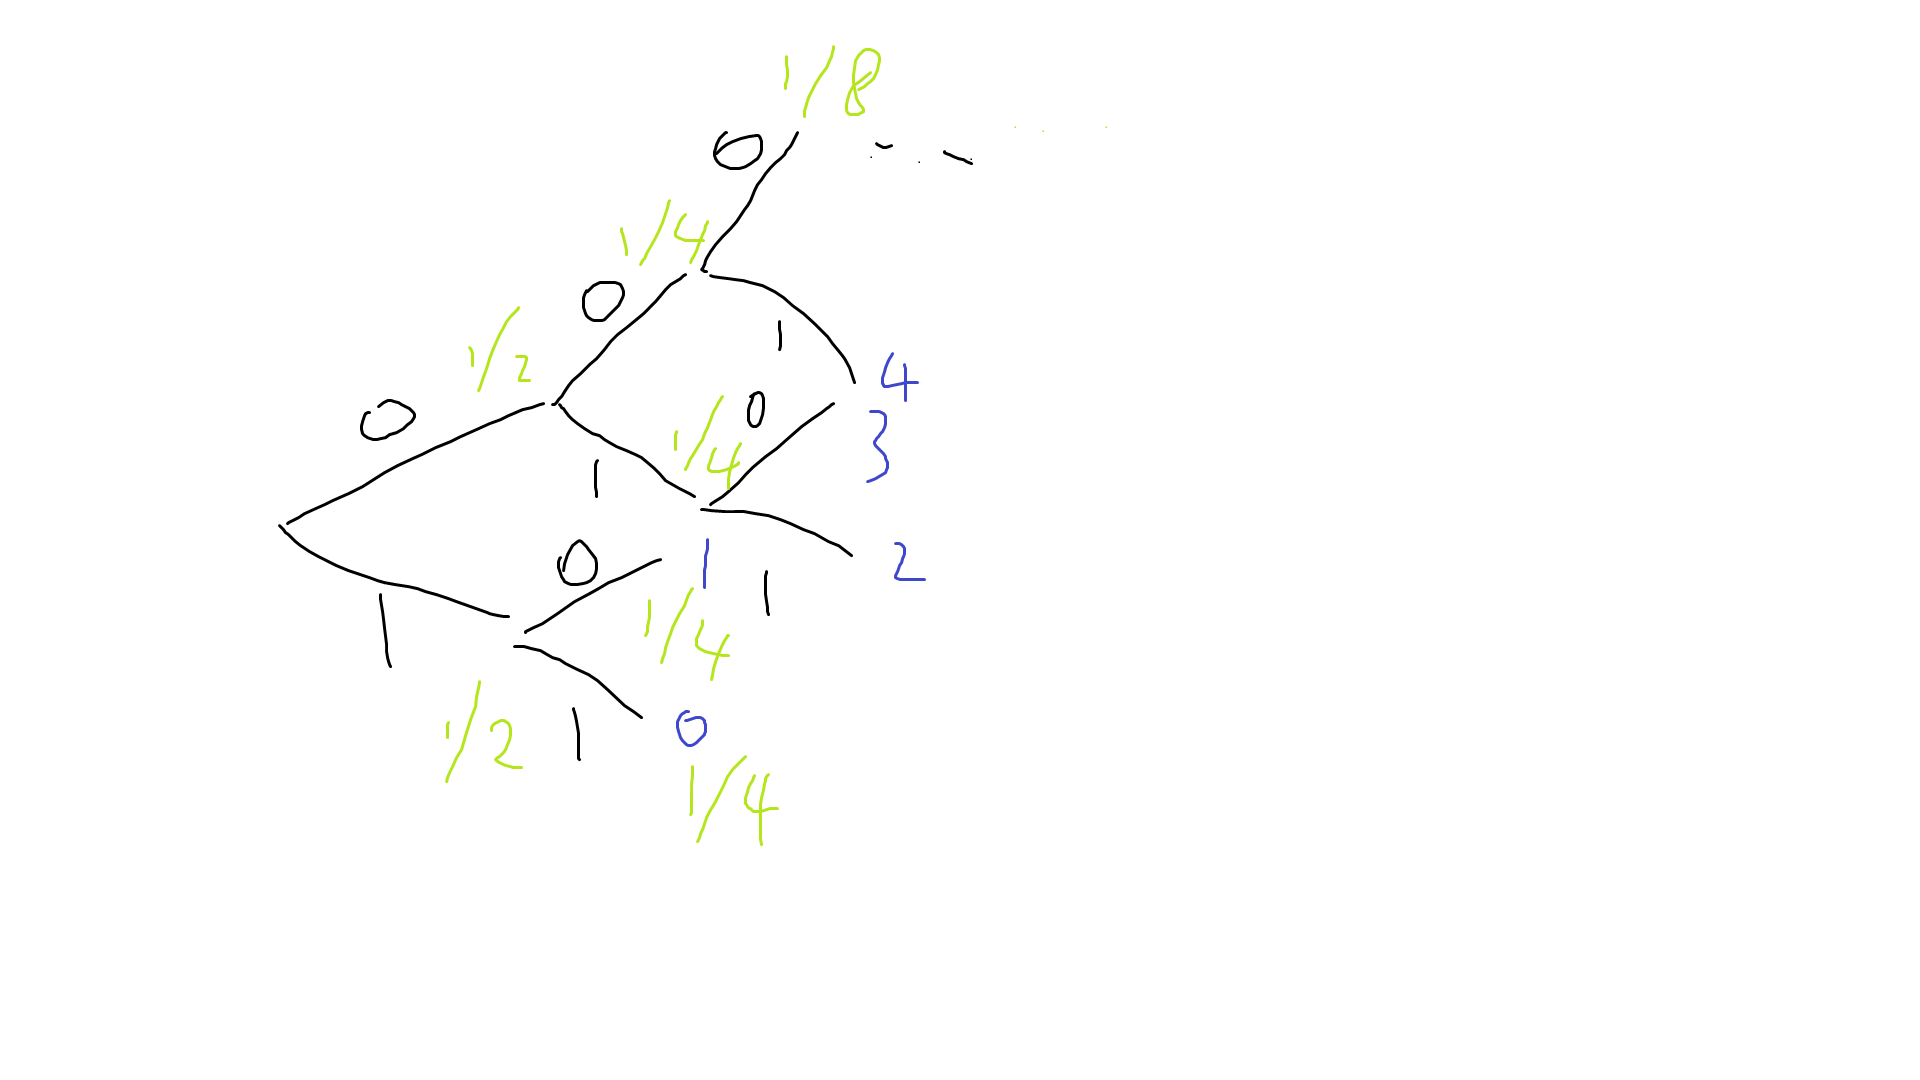
\includegraphics[scale=0.5]{image/CC_01.png}

Conversely, suppose we can construct a prefix-free code with word lengths $s_1,...,s_m$ , wlog $s_1 \leq s_2 \leq ... \leq s_m$. We pick codewords of lengths $s_1,...,$ sequentially ensuring previous codewords are not prefixes. Suppose there is no valid choice for the $r^{th}$ codeword. The constructing the tree as above gives $\sum_{i=1}^{r-1} a^{-s_i} = 1$, contradicting our assumption. So we can construct a prefix-free code.
\end{proof}
\end{thm}

\begin{thm} (1.2, Mcmillan)\\
Every decipherable code satisfies Kraft's inequality.
\begin{proof} (Karush)\\
Let $f:\Sigma_1 \to \Sigma_2^*$ be a decipherable code with word lengths $s_1,...,s_m$, let $s = \max_{1 \leq i \leq m} s_i$. Let $r \in \N$, $$(\sum_{i=1}^m a^{-s_i})^r = \sum_{b = 1}^{rs} b_i a^{-l}$$ where $b_i$ is the number of ways of choosing $r$ codewords of toatl length $l$. $f$ decipherable implies that $b_l \leq |\Sigma_2|^l = a^l$. Thus $(\sum_{i=1}^m a^{-s_i})^r \leq \sum_{l=1}^{rs} a^l a^{-l} = rs$, so $\sum_{i=1}^m a^{-s_i} \leq (rs^{1/r}) \to 1$ as $r \to \infty$. So $\sum_{i=1}^m a^{-s_i} \leq 1$.
\end{proof}
\end{thm}

So we have a corollary: a decipherable code with prescribed word lengths exist iff there exists a prefix-free code with the same word lengths.

So we can restrict our attention to prefix-free codes.

\subsection{Mathematical entropy}
Entropy is a measure of 'randomness' or 'certainty'. Consider a random variable $X$ taking values $x_1,...,x_n$ with probability $p_1,...,p_n$ ($\sum p_i = 1$, $0 \leq p_i \leq 1$). The entropy $H(x)$ is roughly speaking the expected number of tosses of a fair coin needed to simulate $X$ (or the expected number of yes/no questions we need to ask in order to establish the value of $X$).

\begin{eg}
Suppose $p_1 = p_2 = p_3 = p_4 = \frac{1}{4}$. We identify $\{x_1,...,x_4\}$ with $\{HH,HT,TH,TT\}$, so $H(x) = 2$.
\end{eg}

\begin{eg}
$(p_1,p_2,p_3,p_4) = (1/2,1/4,1/8,1/8)$. Then $H(x) = 1/2+1/4 \times 2 + 1/8 \times 3 + 1/8 \times 3=7/4$. So the entropy here is smaller.

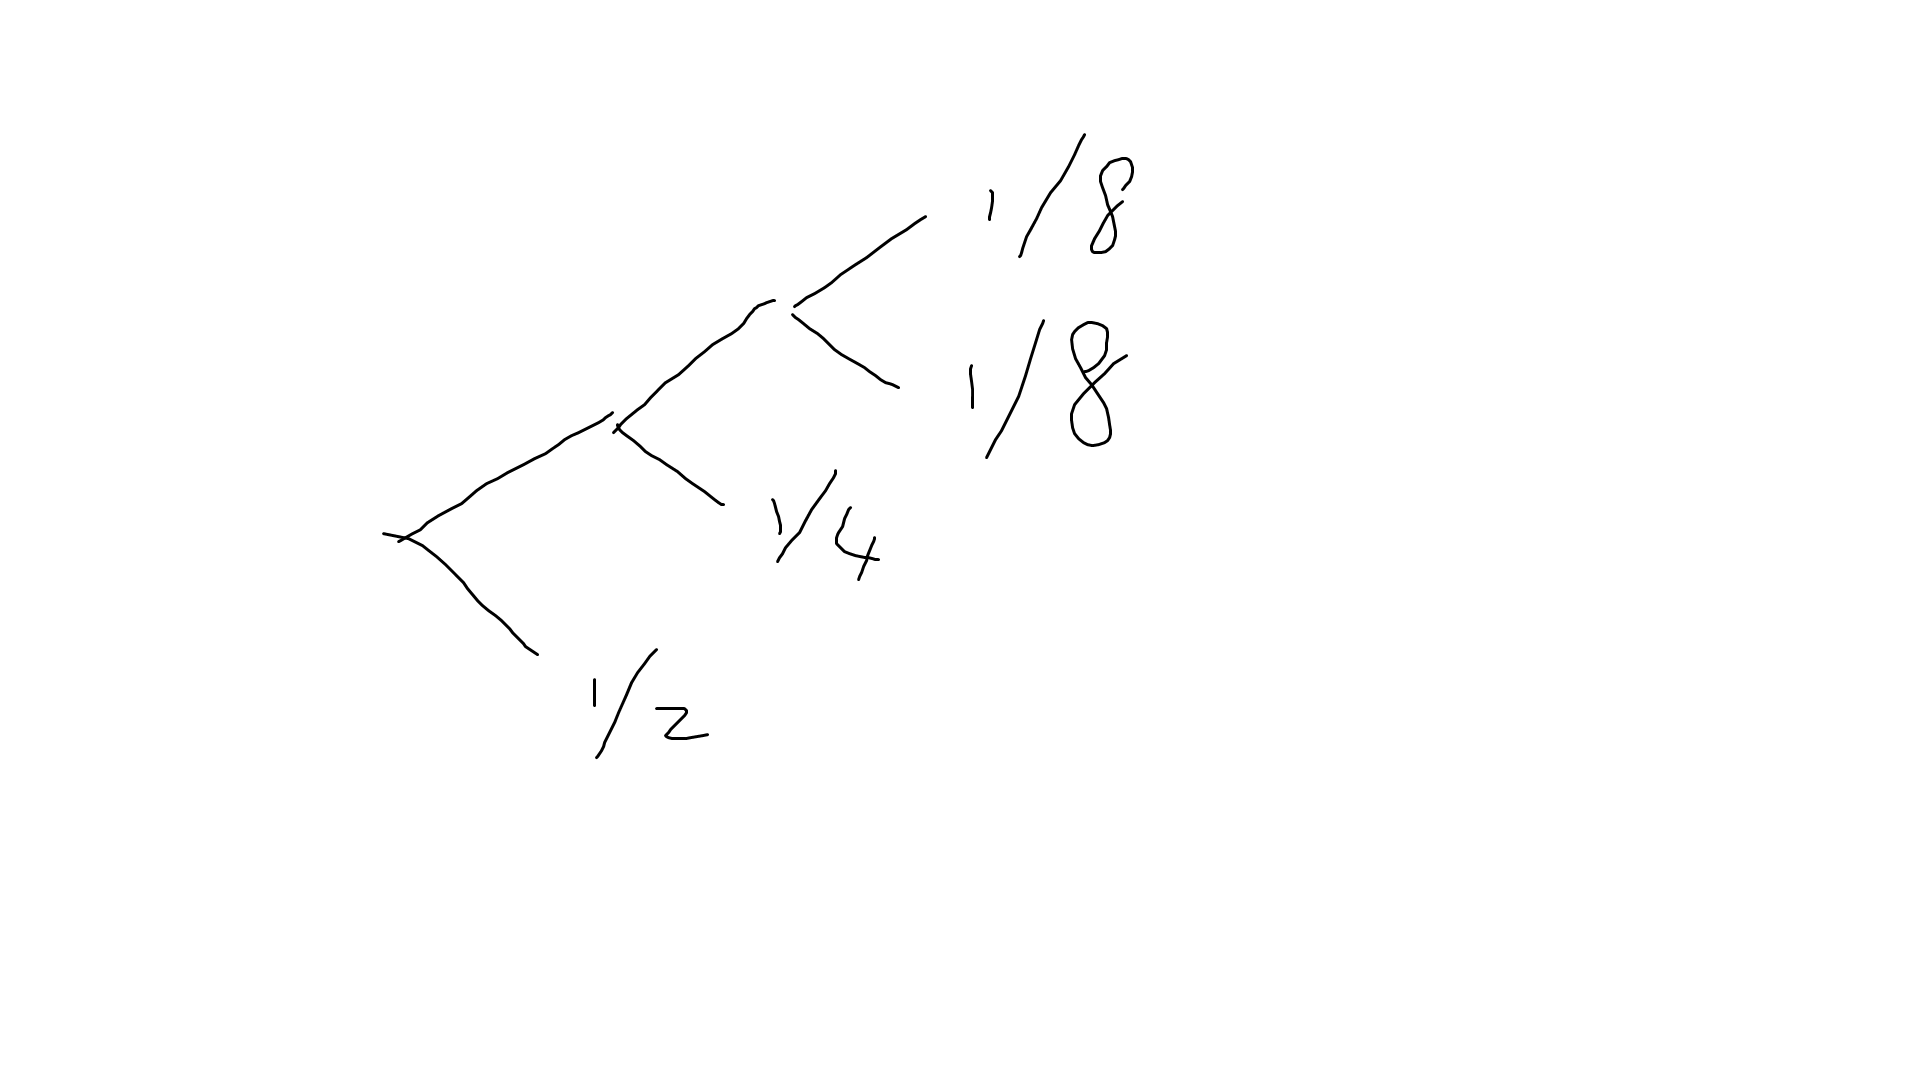
\includegraphics[scale=0.5]{image/CC_02.png}
\end{eg}

So in some sense, there is more randomness in the first example than the second.

\begin{defi} (Entropy)\\
The entropy of $X$, $$H(X) = H(p_1,...,p_n) = -\sum_{i=1}^n p_i \log p_i$$ where, as most of the time in this course, $\log = \log_2$.
\end{defi}

\begin{rem}
(1) If $p_i = 0$, we define $p_i \log p_i = 0$;\\
(2) $H(X) \geq 0$.
\end{rem}

\end{document}
